\documentclass[UTF8]{ctexart}
\usepackage{amsmath,graphicx,tikz,caption,subfigure}
\usepackage[algo2e,ruled,vlined]{algorithm2e}
\usepackage{stfloats}
\usepackage{float}
\usepackage[a4paper]{geometry}
\geometry{left=0.5cm,right=0.5cm,top=0.5cm,bottom=0.5cm}
\title{\textbf{Report3}}
\author{胡琦浩  PB21000235}
\date{\today}

\begin{document}
\maketitle
\section{问题}
在球坐标系($\rho ,\theta ,\varphi $)下,产生上半球面上均匀分布的随机坐标点,给出
其直接抽样方法

\section{方法}
\subsection{数学推导}
在此题中, 我们不妨认定$\rho =1$, 为一个单位球面. 且$\theta\in (0,\frac{\pi}{2})$,$\varphi \in(0,2\pi)$ 

由于点在球面上均匀分布, 则$p(\theta ,\varphi )$为某点在$(\theta ,\varphi )$上的概率即为常数.
\begin{equation}
    p(\theta ,\varphi )=\frac{1}{S_{\text{上半球面}}}=\frac{1}{2\pi}
\end{equation}

设$f(\theta ,\varphi )$为均匀点在球面上分布的概率密度函数, 则显然:
\begin{equation}
    f(\theta ,\varphi )=\frac{sin\theta }{2\pi}
\end{equation}
由于$\theta ,\varphi $相互独立,则:
\begin{equation}
    f(\theta ,\varphi )=\frac{sin\theta }{2\pi}=sin\theta \times \frac{1}{2\pi}=f_1(\theta ) \times f_2(\varphi )
\end{equation}

故:
\begin{equation}
    \xi _1=\int_{0}^{\theta } sint \,dt =1-cos\theta 
\end{equation}
\begin{equation}
    \theta =arccos\xi _1
\end{equation}

\begin{equation}
    \xi_2=\int_{0}^{\varphi } \frac{t}{2\pi} \,dt =\frac{\varphi }{2\pi}
\end{equation}
\begin{equation}
    \varphi =2\pi\xi_2
\end{equation}

\subsection{算法实现}
首先利用第一题产生随机数的方法生成4000个随机数, 前2000个储存到$\xi_1$中, 后2000个储存到$\xi_2$中.然后就可以用直接抽样法,利用公式(5),(7)得到$(\theta ,\varphi )$
的分布,再利用坐标变换公式:
\begin{equation}
    x=sin(\theta)cos(\varphi)
\end{equation}
\begin{equation}
    y=sin(\theta)sin(\varphi)
\end{equation}
\begin{equation}
    z=cos(\theta)
\end{equation}

得到$(x,y,z)$的分布,最后利用python中的matplotlib库画出散点图

\section{实验结果}
\begin{figure}[H]
    \centering
    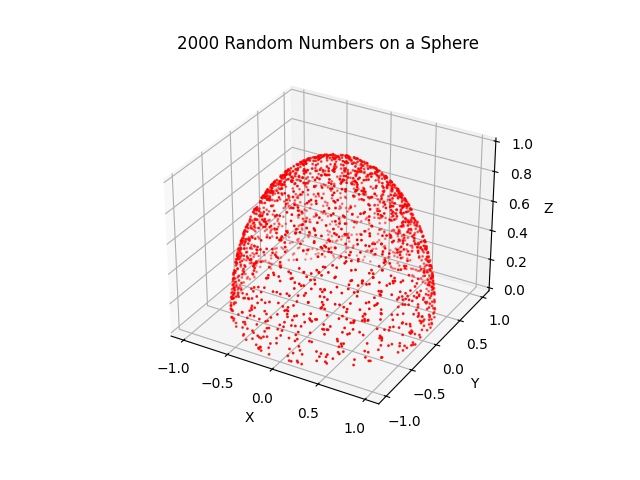
\includegraphics[scale=1]{figure.png}
    \caption{实验结果}
\end{figure}
由图可知, 实验结果较均匀

\section{总结}
由本实验加强了对直接抽样的了解, 并对python作图更加熟练
\end{document}